\documentclass[12pt]{article}
\usepackage[dvipdfm]{graphicx}  %使用图形包
\usepackage{subfig}

\begin{document}
    \section{section 1}
    %基本命令
    
\includegraphics[bb=0 0 300 200]{baby.jpg}  %bb=10 20 100 200 设定 BoundingBox 的左下角在  (10,20),右上角在 (100,200)。

    %图形操作
    %要先生成bb文件才能用,切换到图片路径,使用cmd : ebb baby.jpg 自动生成bb
    
\includegraphics[width=60pt]{baby.jpg}  %v宽度和高度,绝对尺寸,可用任意长度单位。保持图形比例。宽度和高度通常设置一个即可
    
\includegraphics[width=80pt]{baby.jpg}
    
\includegraphics[scale=0.2]{baby.jpg}
    
\includegraphics[width=80pt,height=100pt]{baby.jpg}    
\includegraphics[width=80pt,height=100pt,keepaspectratio]{baby.jpg} %指定图形比例,这样图形宽度和高度都不超过指定参数。
    \\
    %各种旋转,逆时针,其中前三幅图的旋转中心在左下角,后三幅的在图中心。
    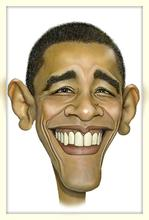
\includegraphics[angle=90]{obama.jpg}
    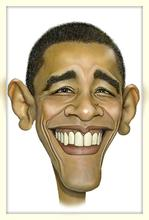
\includegraphics[angle=180]{obama.jpg}
    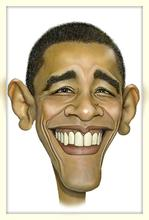
\includegraphics[angle=270]{obama.jpg} \\
    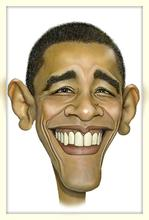
\includegraphics[angle=90,origin=c]{obama.jpg}
    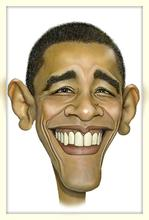
\includegraphics[angle=180,origin=c]{obama.jpg}
    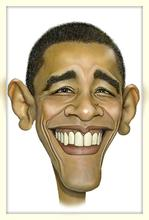
\includegraphics[angle=270,origin=c]{obama.jpg} \\

    %文件名和搜索路劲
    \DeclareGraphicsExtensions{.eps ,.mps ,.pdf ,.jpg ,.png}    %指定后缀列表让编译程序自行查找
    \DeclareGraphicsRule {*}{eps}{*}{}  %指出未知后缀的都是 EPS
    %设置缺省搜索路径,分别使用了绝对路径、相对路径、多个路径
    \graphicspath{{c:/secret -garden/}}
    \graphicspath{{./}}
    \graphicspath{{one-little/}{two-little/}{three-little-indians/}}

    %figure环境
    %htbp这几个字母分别代表 here, top, bottom, ìoat page,也就是就这里、页顶、页尾、浮动页 (专门放浮动环境的单独页面) 。这几个字母的任意组合,四个母都写上表示放哪里都无所谓;一般不推荐单独使用 h,
    \begin{figure}[htbp]
        \centering  %居中
        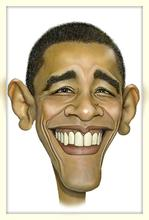
\includegraphics{obama.jpg}
        \caption{Obama SB}  %图的题注,会自动加上编号
        \label{fig:myphoto} % \label 应该放在标题之后,否则引用时指向的是前一个结构对象
    \end{figure}

    %插入多个图
    %并排放,共享标题
    \begin{figure}[htbp]
        \centering
        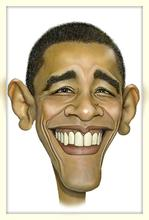
\includegraphics{obama.jpg}
        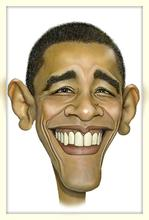
\includegraphics{obama.jpg}
        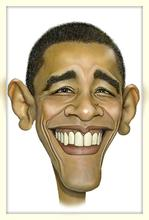
\includegraphics{obama.jpg}
        \caption{obama is sb}
    \end{figure}

    %并排放,各有标题, 需要使用minipage
    \begin{figure}[htbp]
        \centering
        \fbox{%
        \begin{minipage}{149pt}  %括号中指定宽度...使用fbox显示一个边框..
            \centering
            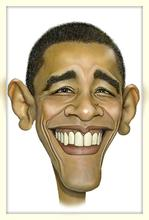
\includegraphics{obama.jpg}
            \caption{sb1}
        \end{minipage}%
        }
        \hspace{20pt}%
        \begin{minipage}{149pt}
            \centering
            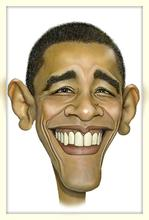
\includegraphics{obama.jpg}
            \caption{sb2}
        \end{minipage}
    \end{figure}

    %并排摆放,共享标题,各有子标题,使用subfig宏包的subfloat
    \begin{figure}[htbp]
        \centering
        \subfloat[xxoo]{
            \label{fig:subfig_a}
            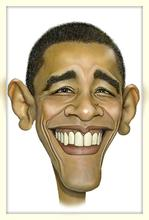
\includegraphics{obama.jpg}
        }
        \hspace{10pt}%
        \subfloat[ooxxxxxxxxxxxxxxxxxx]{
            \label{fig:subfig_b}
            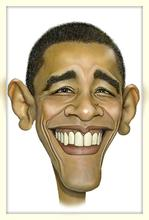
\includegraphics{obama.jpg}
        }
        \caption{sb xxoo}
        \label{fig:subfig}
    \end{figure}

    %改进子图方法
    %\subfloat 命令缺少宽度参数,而子标题最多只能和子图一样宽,太长的话会出现折行。为了避免子标题折行,我们可以在 \subfloat 里再嵌套个 minipage,因为后者是有宽度的
    \begin{figure}[htbp]
        \centering
        \subfloat[xxoo]{
            \label{fig:subfig_a}
            \begin{minipage}[t]{149pt}
                \centering
                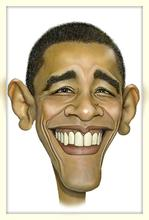
\includegraphics{obama.jpg}
            \end{minipage}
        }
        \hspace{10pt}%
        \subfloat[ooxxxxxxxxxxxxxxxxxx]{
            \label{fig:subfig_b}
            \begin{minipage}[t]{149pt}
                \centering
                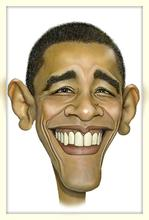
\includegraphics{obama.jpg}
            \end{minipage}
        }
        \caption{sb xxoo}
        \label{fig:subfig}
    \end{figure}


\end{document}
